\documentclass[journal,10pt,twocolumn]{article}
\usepackage{graphicx}
\usepackage[margin=0.5in]{geometry}
\usepackage[cmex10]{amsmath}
\usepackage{array}
\usepackage{booktabs}
\usepackage{mathtools}
\title{\textbf{Optimization Assignment - 2}}
\author{VAMSI SUNKARI}
\date{September 2022}



\let\vec\mathbf
\newcommand{\myvec}[1]{\ensuremath{\begin{pmatrix}#1\end{pmatrix}}}
\newcommand{\mydet}[1]{\ensuremath{\begin{vmatrix}#1\end{vmatrix}}}
\providecommand{\brak}[1]{\ensuremath{\left(#1\right)}}
\providecommand{\lbrak}[1]{\ensuremath{\left(#1\right.}}
\providecommand{\rbrak}[1]{\ensuremath{\left.#1\right)}}
\providecommand{\sbrak}[1]{\ensuremath{{}\left[#1\right]}}

\begin{document}

\maketitle
\paragraph{\textit{Problem Statement} - Amongst all open (from the top) right circular cylindrical boxes of volume $125\pi cm^{3}$, find the dimensions of the box which has the least surface area.}
\section*{\large Solution}
\subsection{\textbf{Considerations}}


\begin{tabular}{|c|c|}
 \hline
 \textbf{Symbol}&\textbf{Description}\\
 \hline
 r&radius of cylinder\\
 \hline
 h&height of cylinder\\
\hline
\end{tabular}\\
    Volume of the cylinder
    \begin{equation}
        V = \pi r^2 h
    \end{equation}
    \begin{equation}
        S = 2\pi rh + \pi r^2
    \end{equation}
    \begin{equation}
        S = \frac{250 \pi}{r} + \pi r^2 
    \end{equation}
    \textbf{Minima using conventional method}
    \begin{equation}
        \frac{dS}{dr} = \frac{-250 \pi}{r^2} + 2 \pi r
    \end{equation}
    \begin{equation}
        \frac{-250 \pi}{r^2} + 2 \pi r = 0
    \end{equation}
    \begin{equation}
        r^3 = 125
    \end{equation}
    
    \begin{equation}
        r = 5 cm
    \end{equation}
    \begin{equation}
	    V=\pi r^2   h=125\pi
    \end{equation}
    \begin{equation}
	    h=\frac{125}{r^2}=5 cm
    \end{equation}
	
\subsection*{\normalsize Gradient descent}
Using gradient descent method we can find its minima ,
    \begin{align}
        x_{n+1} &= x_n - \alpha \nabla f(x_n) \\
        \implies x_{n+1} &= x_n - \alpha \brak{\frac{250 \pi}{r^2} + 2 \pi r}
    \end{align}
   
Taking $x_0=0.1,\alpha=0.001$ and precision = 0.00000001, values obtained using python are:
    
    \begin{align}
        \boxed{\text{Minima} = 235.61}\\
        \boxed{\text{Minima Point} = 5.00}
    \end{align}
\begin{figure}[t]
 \centering
 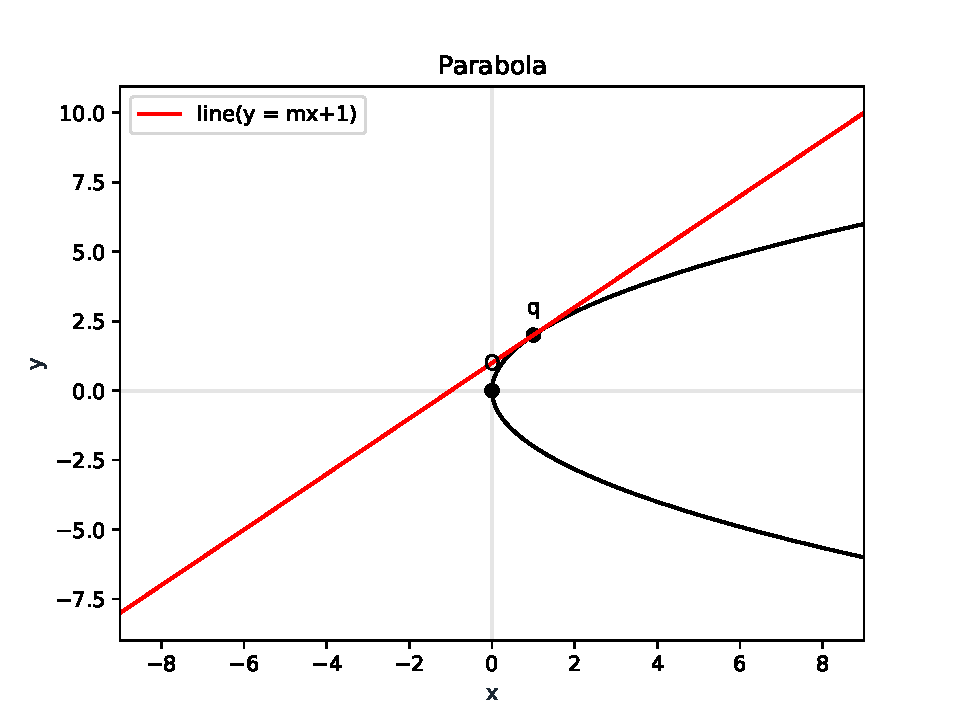
\includegraphics[width=1\columnwidth]{im.pdf}
 \caption{Graph of Surface area}
 \label{fig:graph_fx}
\end{figure}

\end{document}
